\paragraph{Additional relations}
\begin{enumerate}
	\item Circular orbit has $v = \sqrt{\frac{GM_*}{r}}$. So from ($e=0$):
	$$\frac{E}{m} = \frac{1}{m} \left[ \frac{1}{2}mv^2 + \left( -G\frac{M_*m}{r} \right) \right] = \frac{1}{2}v^2 - \frac{GM_*}{r}$$
	by substituting we get
	$$E = E_k+U_G = \frac{1}{2}U_G = -E_k$$
	\item In elliptical orbit $E_k$ and $U_G$ are changing in time. It is possible to define average values over orbit:
	$$E = \frac{1}{2}\bar{U}_G = - \bar{E}_k$$
	Calculation shows:
	$$\bar{U}_G = -\frac{GM_*m}{a}$$
	$$E = -\frac{1}{2}\frac{GM_*m}{a}$$
	\item $e=\frac{r_{max}-r_{min}}{r_{max}+r_{min}}$, where $r_{max}=a(1+e)$ and $r_{min}=a(1-e)$.
	\item For ellipse, substituting $\frac{E}{m} = -\frac{1}{2}\frac{GM_*}{a}$ in expression for $e$ we get:
	$$\frac{J}{m} = \sqrt{GM_*a(1-e^2)}$$ and
	$$\left( \frac{J}{m} \right)^2\frac{1}{GM_*} = a(1-e^2)$$
	\item For ellipse 
	$$\frac{1}{2}\frac{GM_*}{a}= \frac{v^2}{2}-\frac{GM_*}{r}$$
	or
	$$\frac{1}{a} = \frac{2}{r} - \frac{v^2}{GM_*}$$
\end{enumerate}

\paragraph{Third law of Kepler}
We found that $\frac{d\vec{S}}{dt} = \frac{\vec{J}}{2m}$ which is implied from conservation of angular momentum.

Integral on time of cycle:

$$\oint dS = \int_0^T \underbrace{\frac{J}{2m}}_{\parbox{1cm}{\centering \scriptsize const}} dt = \frac{J}{2m}T$$

By substituting $b=a\sqrt{1-e^2}$ and $\frac{J}{m}$ we get:

$$T^2 = \left( \frac{2m}{J} \right)^2 S^2 = \frac{4}{GM_*a(1-e^2)}\underbrace{\pi^2 a^2 \left[ a^2 \left( 1 - e^2 \right) \right]}_{\parbox{2cm}{\centering \scriptsize ellipse area}}$$

And we get third law:

$$T^2 = \frac{4\pi^2}{GM_*}a^3$$

\subparagraph{Reduced mass}
When $m_2 \centernot\ll m_1$:
\begin{center}
	\includegraphics[width=\linewidth]{./lect16/pic1.png}
\end{center}
$$\vec{R}_{1cm} = \frac{m_2}{m_1+m_2}a\hat{r}$$
$$\vec{R}_{2cm} = \frac{m_1}{m_1+m_2}a\left(-\hat{r}\right)$$

We are at circular orbit. Lets compare centrifugal force with gravitational force:
$$\left| F_{cen} \right| = \left| F_{g} \right|$$ 
At second mass:
$$m_2\omega^2 R_{2cm} = \frac{Gm_1m_2}{a^2}$$
By substituting $R_{2cm}$:
$$\omega^2 \frac{m_1}{m_1+m_2}a = \frac{Gm_1}{a^2}$$
$$\omega = \sqrt{\frac{G\left(m_1+m_2\right)}{a^3}}$$

Now substitute $T = \frac{2\pi}{\omega}$:
$$T^2 = \frac{2\pi a^3}{G\left( m_1+m_2 \right)}$$

Which is third law of Kepler.

Angular momentum:

$$\left|\vec{J}\right| = m_1R_{1cm}^2\omega+ m_2R_{2cm}^2\omega$$

Direction of $\vec{J}$ is perpendicular to plane of movement.

$$J = \frac{m_1m_2^2}{\left(m_1+m_2\right)^2}a^2\omega+ \frac{m_2m_1^2}{\left(m_1+m_2\right)^2}a^2\omega$$

Acquiring:

$$J = \frac{m_1m_2}{\left( m_1+m_2 \right)}a^2\omega$$

Define reduced mass - $\mu = \frac{m_1m_2}{\left( m_1+m_2 \right)}$ resulting in:

$$J  = \mu a^2 \omega$$

Kinetic energy is:

$$E_k = \frac{1}{2} m_1\left( R_{1cm}\omega \right)^2+\frac{1}{2} m_2\left( R_{2cm}\omega \right)^2$$

Acquiring:

$$E_k = \frac{1}{2}\mu a^2\omega^2$$

And total energy:

$$E = \frac{1}{2}\mu a^2\omega^2 - \frac{Gm_1m_2}{a}$$
$$E = \frac{1}{2}\mu a^2\omega^2 - \frac{G\left(m_1+m_2\right)\mu}{a}$$

When $m_1 \centernot\ll m_2$ we replace $m$ with $\mu$ and $M_*$ with $m_1+m_2$.

\paragraph{Rigid body} We talk about rigid body rotating around constant axis. $\omega$ is same for each part of body. We consider only case when $\vec{\omega}$ and $\vec{J}$ are in same direction.


\begin{center}
	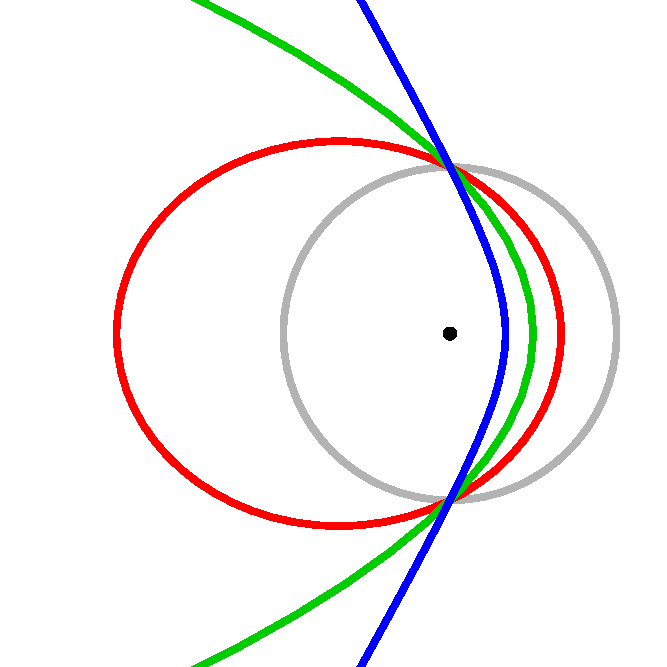
\includegraphics[width=0.1\linewidth]{./lect16/pic2.png}
\end{center}

$$\vec{v} = \vec{\omega} \times \vec{r}$$
In point $p$ there is mass $m$ and its contribution to total angular momentum is:

$$\vec{j}_p = m_p \vec{r}_p \times \vec{v}_p$$

We work with $\hat{\omega} = \hat{J}$ which is not always true. Then

$$\left[\vec{r}_i \times \left(\vec{\omega}_i \times \vec{r_i}\right)\right]_{\hat{J}} = \left| \vec{r}_i \times \left(\vec{\omega}_i \times \vec{r_i} \right) \right| \sin \theta \hat{J} = \left( r_i \sin \theta \right)^2 \vec{\omega} = d^2 \vec{\omega}$$
 Total angular momentum is:
$$\vec{J} = \sum_i \vec{j}_i = \sum_i m_i \vec{r}_i \times \vec{v}_i =\sum_i m_i \vec{r}_i \times \left(\vec{\omega}_i \times \vec{r_i}\right) = \sum_i m_i d_i^2 \vec{\omega}$$

where $d_i = r_i \sin \theta_i$ is distance from rotation axis. We get

$$\vec{J} = \vec{\omega} \sum_i m_id_i^2$$

And kinetic energy of the body:

$$E_k = \sum_i \frac{1}{2} m_i v_i^2 = \sum_i \frac{1}{2} m_i \left( \vec{\omega} \times \vec{r}_i \right) \left( \vec{\omega} \times \vec{r}_i \right) = \sum_i \frac{1}{2} m_i d_i^2 \omega^2$$

We got:

$$E_k = \frac{1}{2}\left( \sum_i m_i d_i^2 \right) \omega^2$$

\paragraph{Conclusion} For our case we got:

$$\vec{J} = I\vec{\omega}$$
$$E_k = \frac{1}{2} I \omega^2$$

Where $I$ is moment of inertia which we defined as:

$$I = \sum m_i d_i^2$$

Moment of inertia depends on choice of axis of rotation (both place and direction).

For contiguous body we replace mass with small mass $m_i \to dm = \rho dV$.

$$I = \int \underbrace{R^2}_{\parbox{1.5cm}{\centering \scriptsize distance of dV from axis}} \underbrace{\rho dV}_{\parbox{1cm}{\centering \scriptsize dm}} $$